\chapter{Reduced Electronic Density Distribution} \label{ED}

\section{Self-consistent Poisson-Schrodinger Solver} \label{sec:model}

%\subsection{What Reddening Law Fits Better?}\label{sec:DIC}


\section{Electronic Distribution in Nanowires} \label{sec:spectra}

Figure 8 (C) shows the FDTD-simulated electric field density of a hexagonal
nanowire at y cross section (top) and x cross section (bottom). The photon
energy of this mode shown as the insets of Fig. 8(C) is concentrated primarily
along the 6 corners and secondarily along the facets with little light in the
3D core of GaAs. Hence, we suggest that the fortuitous spatial overlap of the
resonant optical modes on reduced dimensional electronic wavefunctions plays a
significant role in the remarkable optoelectronic properties of core-shell
nanowires. Restated, the superposition of the photon modes  on reduced
electronic states that form on the facets and vortices of the hexagonal CSNWs
strongly enhances both upward and downward transition rates.  Thus, the reduced
dimensionality transition rate distinguishes the core-shell nanostructure from
the optically equivalent structures of Fig. 6 due to its significantly modified
rate management. These nanostructures are not only excellent optical cavities,
but despite their large size also provide the right reduced dimensional
electronic structures which enhance optoelectronic interactions.  It should be
noted the present analysis is for direct optical transitions; although it can
be extended to incorporate k-vector changes as in phonon scattering, other
important factors such as many-body interactions need to be included in a
comprehensive analysis.

\subsection{Cylindrical Core-Shell Nanowire}

\subsection{Hexagonal Core-shell Nanowire} \label{sec:indv_lines}

\begin{figure}
  \caption{One Dimensional Electron Charge with band bending}
  \centering
  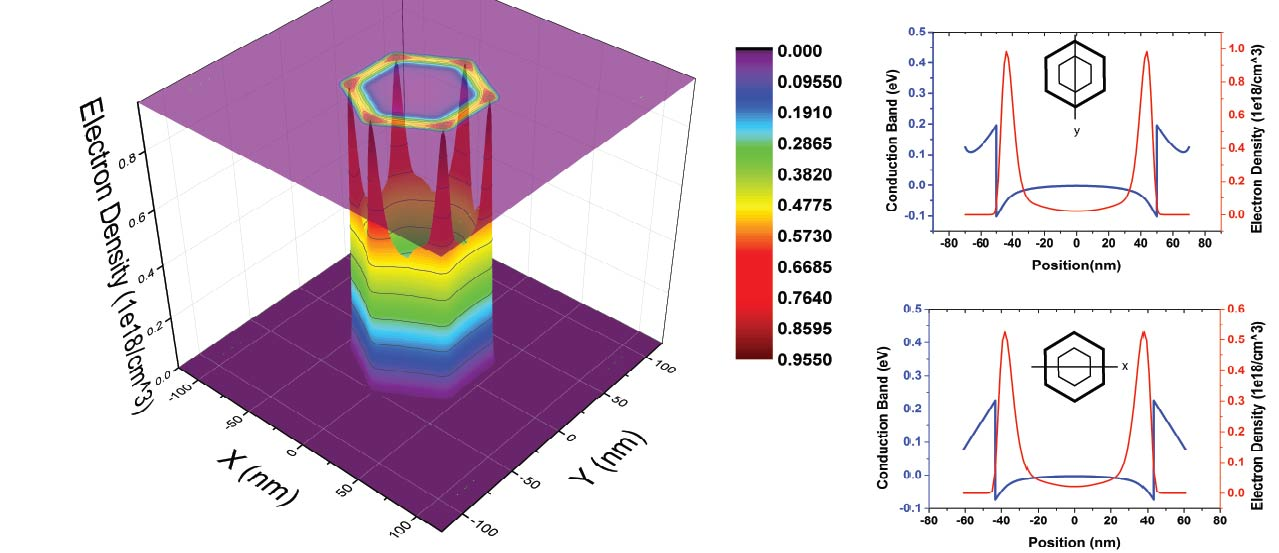
\includegraphics[width=\textwidth]{pictures/ED/1DCharge}
  \label{1DCharge}
\end{figure}

\begin{figure}
  \caption{Two Dimensional Electron Charge with band bending}
  \centering
  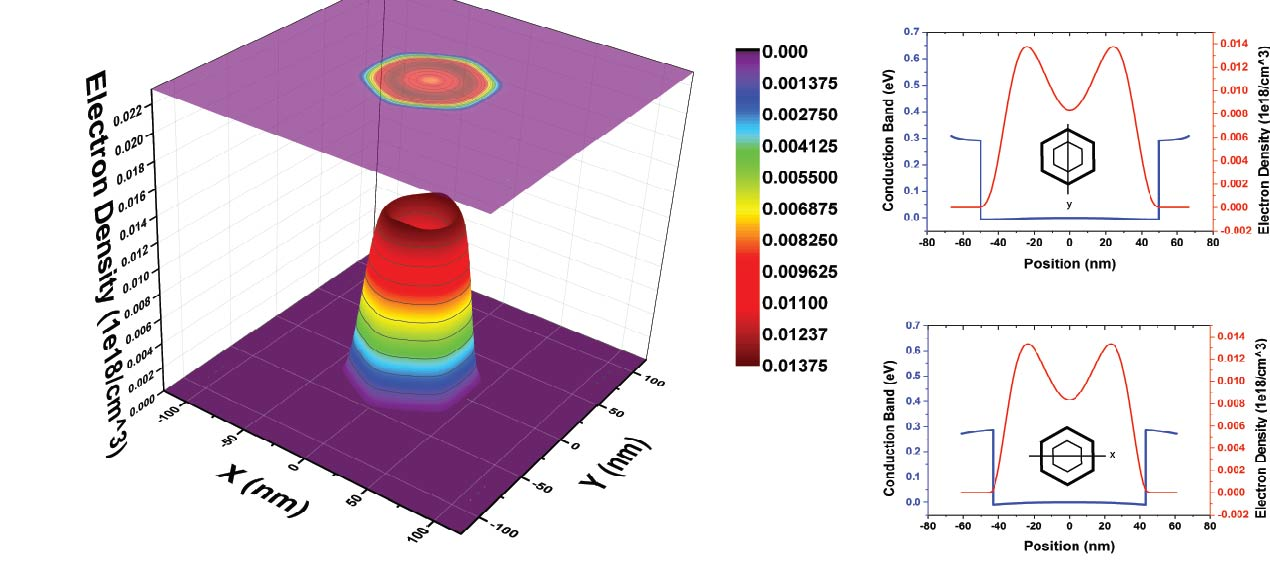
\includegraphics[width=\textwidth]{pictures/ED/2DCharge}
  \label{2DCharge}
\end{figure}

\begin{figure}
  \caption{Three Dimensional Electron Charge with band bending}
  \centering
  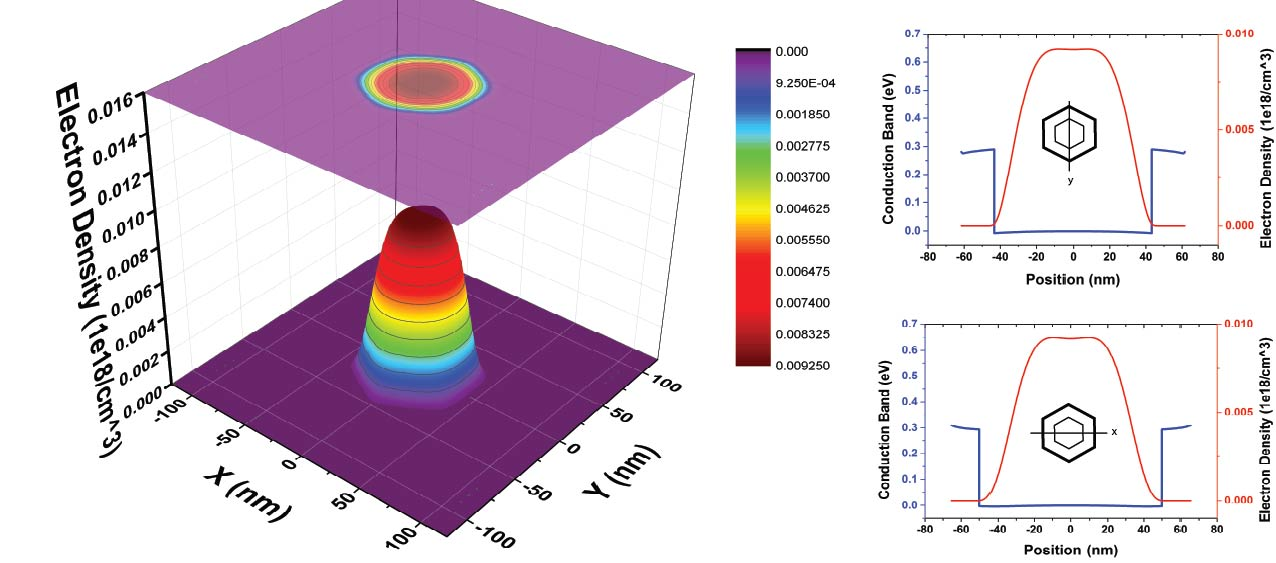
\includegraphics[width=\textwidth]{pictures/ED/3DCharge}
  \label{3DCharge}
\end{figure}

\begin{figure}
  \caption{Photon Charge Distribution}
  \centering
  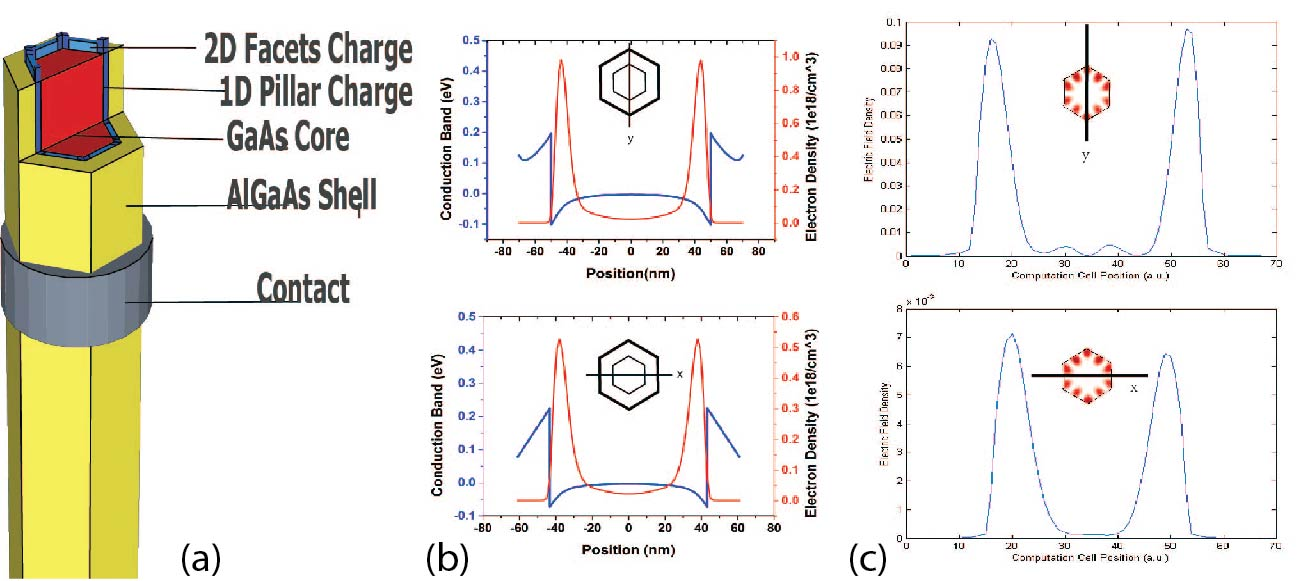
\includegraphics[width=\textwidth]{pictures/ED/Photoncharge}
  \label{PhotonCharge}
\end{figure}

\section{Conclusions} \label{sec:conclusions}

